%% START FAVITES SUPPLEMENT
\chapter{Supplemental Material for Chapter~\ref{chap:favites}}
\label{chap:favites-sup}
\clearpage

\begin{table}[!ht]
\caption[Comparison with Existing Simulation Tools]{Comparison with Existing Simulation Tools}
\vspace{-0.25in}
\begin{center}
\begin{tabular}{|P{0.8in}|P{0.5in}|P{0.8in}|P{0.8in}|P{0.6in}|P{0.8in}|P{0.8in}|}
\hline
 & \textbf{epinet} & \textbf{TreeSim} & \textbf{outbreaker} & \textbf{seedy} & \textbf{PANGEA} & \textbf{FAVITES} \\
\hline
\textbf{Contact Network} & Fixed & Complete & Complete & Complete & Fixed & Any \\
\hline
\textbf{Trans. Network} & Fixed & Fixed & Fixed & Fixed & Fixed & Any\\
\hline
\textbf{Sampling} & N/A & Fixed or \newline Sequential & Fixed & Uniform & Fixed & Any \\
\hline
\textbf{Phylogeny} & None & Fixed & Fixed & Fixed & Coalescent & Any \\
\hline
\textbf{Mutation Rate} & N/A & N/A & Constant & Constant & Fixed & Any \\
\hline
\textbf{Sequences} & None & None & Fixed & Fixed & Fixed & Any \\
\hline
\textbf{Sequencing} & N/A & N/A & No & No & No & Any \\
\hline
\end{tabular}
\end{center}
\label{tab:favites-comparison}
\end{table}

\begin{table}[!ht]
\caption[Post-Validation Tools]{Post-Validation Tools}
\vspace{-0.25in}
\begin{center}
\begin{tabular}{|P{2.3in}|P{3.7in}|}
\hline
\textbf{Name} & \textbf{Description}  \\
\hline
compare\_contact\_networks.py & Compare the degree distributions of a given simulated contact network against a reference contact network \\
\hline
compare\_trees.py & Compare the distributions of all branch lengths, internal branch lengths, terminal branch lengths, and root-to-tip distances between a given simulated tree against a given reference tree \\
\hline
distribution\_distance.py & Compute a distance between two distributions given samples from each \\
\hline
ltt.py & Create a \gls{LTT} plot from one or more Newick trees \\
\hline
sequence\_score\_profile\_HMM.py & Score a given sequence dataset against a given profile \gls{HMM} \\
\hline
\end{tabular}
\end{center}
\label{tab:favites-post-validation}
\end{table}

\begin{table}[!ht]
\caption[Helper Scripts]{Helper Scripts}
\vspace{-0.25in}
\begin{center}
\begin{tabular}{|P{2.75in}|P{3.25in}|}
\hline
\textbf{Name} & \textbf{Description}  \\
\hline
clean\_labels.py & For each read of the given sequence file or each leaf of a given phylogenetic tree, remove everything from the label except for the contact network individual's name \\
\hline
cluster\_previous\_time.py & Given a clustering from the simulation end time, a FAVITES-format transmission network, and a time, remove individuals who were not infected at the given time and output the resulting clusters \\
\hline
cn\_adjacency\_matrix\_to\_favites.py & Convert a given contact network from a binary adjacency matrix to the FAVITES format \\
\hline
degree\_stats.py & Given a contact or transmission network, compute various statistics of the node degree distribution \\
\hline
FAVITES2GEXF.py & Convert a FAVITES contact network and transmission network to the GEXF format \\
\hline
PANGEA\_transmissions\_to\_FAVITES.py & Convert a PANGEA transmission network into the FAVITES edge-list format \\
\hline
patristic\_distances.py & Given a phylogenetic tree, compute the pairwise distances between leaves and output the resulting distance matrix as a CSV file \\
\hline
scale\_tree.py & Given a phylogenetic tree (in the Newick format), scale all branches \\
\hline
score\_clusters.py & Score a given query clustering against a given true reference clustering \\
\hline
tn93\_to\_clusters.py & Convert tn93 output to the Cluster Picker clustering format \\
\hline
\end{tabular}
\end{center}
\label{tab:favites-helper}
\end{table}

\begin{table}[!ht]
\caption[HIV Simulation Parameters (epidemiological model)]{HIV Simulation Parameters (epidemiological model)}
\vspace{-0.25in}
\begin{center}
\begin{tabular}{|P{2in}|P{1.9in}|P{1.9in}|}
\hline
 & \textbf{San Diego} & \textbf{Uganda} \\
\hline
\textbf{CN Model} & \gls{BA} & \gls{BA} \\
\hline
\textbf{Expected Degree} & 4 & 4 \\
\hline
\textbf{Number of Seeds} & 1,500 & 15,000 \\
\hline
\textbf{$\lambda_{AU\rightarrow CU}$} (year$^{-1}$) & 8.667 & 8.667 \\
\hline
\textbf{$\lambda_{AT\rightarrow CT}$} (year$^{-1}$) & 4.333 & 4.333 \\
\hline
\textbf{$\lambda_{U\rightarrow T}$} (year$^{-1}$) & 1 & 1 \\
\hline
\textbf{$\lambda_{T\rightarrow U}$} (year$^{-1}$) & 1 & 0.48 \\
\hline
\textbf{$\lambda_{S,AU}$} (year$^{-1}$) & 0.1125 & 0.1125 \\
\hline
\textbf{$\lambda_{S,AC}$} (year$^{-1}$) & 0.0225 & 0.0225 \\
\hline
\textbf{$\lambda_{S,AT}$} (year$^{-1}$) & 0.005625 & 0.005625 \\
\hline
\textbf{$\lambda_{S,CT}$} (year$^{-1}$) & 0 & 0 \\
\hline
%\textbf{Rate from Acute Treated to Chronic Treated} & 
\end{tabular}
\end{center}
\label{tab:favites-params-epi}
\end{table}

\begin{table}[!ht]
\caption[HIV Simulation Parameters (evolutionary model)]{HIV Simulation Parameters (evolutionary model)}
\vspace{-0.25in}
\begin{center}
\begin{tabular}{|P{2in}|P{1.9in}|P{1.9in}|}
\hline
 & \textbf{San Diego} & \textbf{Uganda} \\
\hline
\textbf{Seed Height} (years) & 25 & 25 \\
\hline
\textbf{Seed Rate} & $1 + e^{-t^2}$ & $1 + e^{-t^2}$ \\
\hline
\textbf{Population Growth} & 2.852 & 2.852 \\
\hline
\textbf{v.T50} & -2 & -2 \\
\hline
\textbf{Mutation Rate Location} & 0.0008 & 0.001 \\
\hline
\textbf{Mutation Rate Scale} & 0.0005 & 0.0005 \\
\hline
\textbf{\gls{GTR} $\pi_A$} & 0.392 & 0.377 \\
\hline
\textbf{\gls{GTR} $\pi_C$} & 0.164 & 0.172 \\
\hline
\textbf{\gls{GTR} $\pi_G$} & 0.212 & 0.210 \\
\hline
\textbf{\gls{GTR} $\pi_T$} & 0.232 & 0.241 \\
\hline
\textbf{\gls{GTR} $\pi_{AC}$} & 1.812 & 1.388 \\
\hline
\textbf{\gls{GTR} $\pi_{AG}$} & 9.934 & 7.017 \\
\hline
\textbf{\gls{GTR} $\pi_{AT}$} & 0.718 & 0.736 \\
\hline
\textbf{\gls{GTR} $\pi_{CG}$} & 0.971 & 0.594 \\
\hline
\textbf{\gls{GTR} $\pi_{CT}$} & 9.934 & 8.618 \\
\hline
\textbf{\gls{GTR} $\pi_{GT}$} & 1 & 1 \\
\hline
\textbf{$\alpha$} ($\Gamma$ shape) & 0.405 & 0.449 \\
\hline
\end{tabular}
\end{center}
\label{tab:favites-params-evo}
\end{table}

\begin{figure}[h] 
\centering
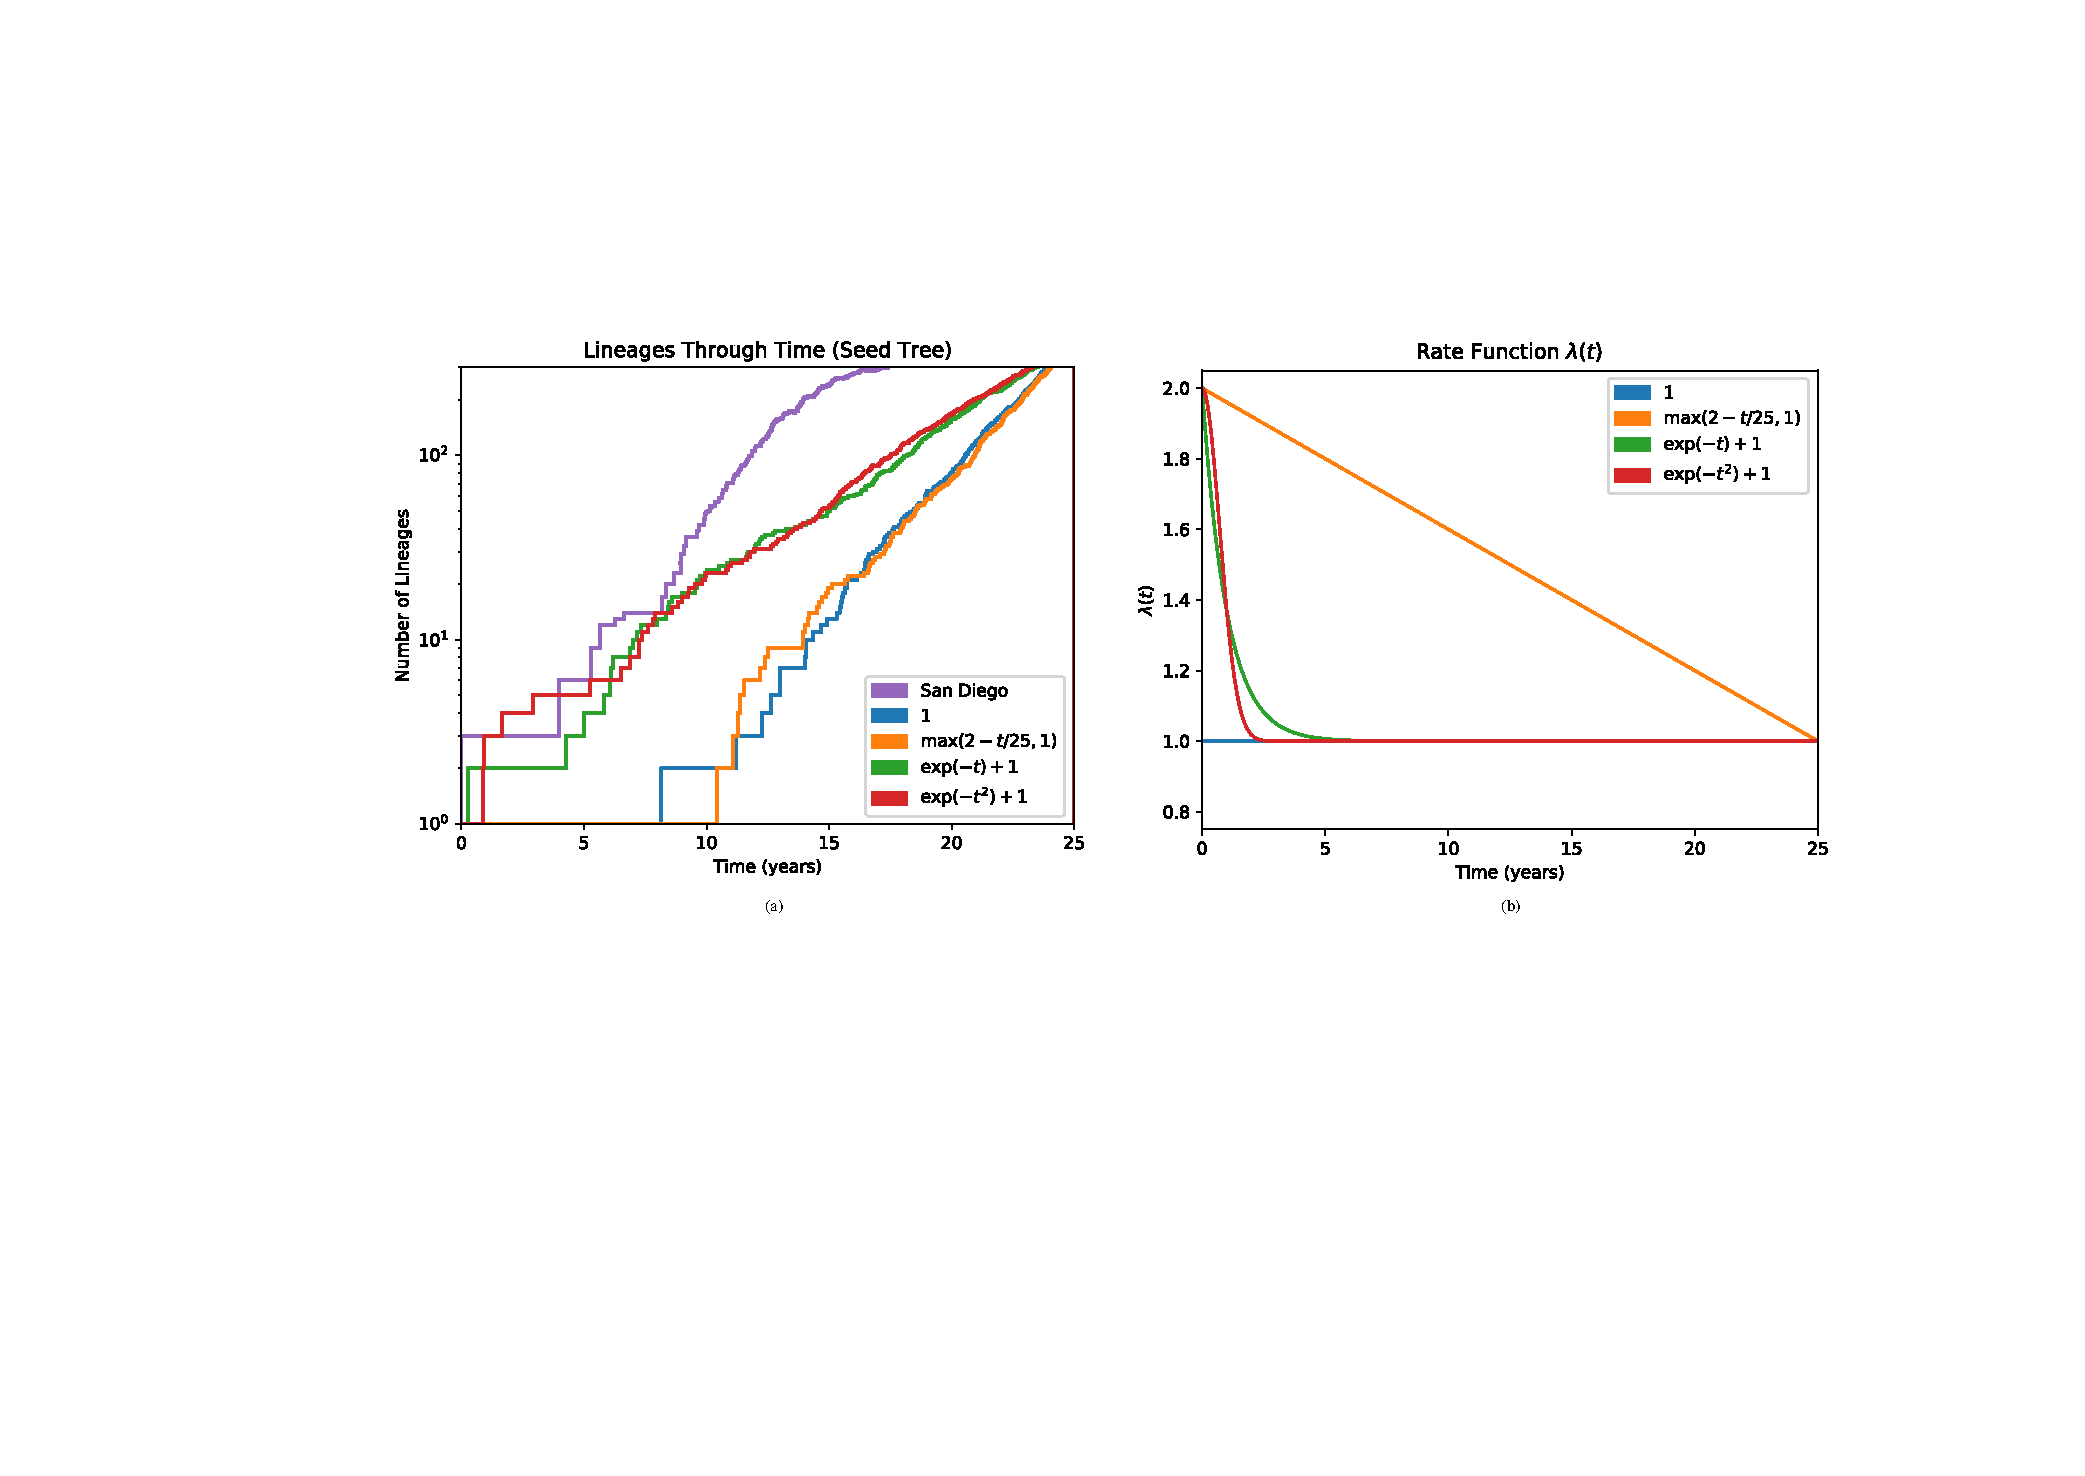
\includegraphics[width=\textwidth]{figs/favites-seed-tree}
\caption[Seed Tree]
{(a) \gls{LTT} plot of the first 25 years of the dated San Diego tree along with multiple potential rate functions for the non-homogeneous Yule model~\cite{LeGat2016}, and (b) plots of the rate functions. Because HIV trees have more short branches than normal Yule models (i.e., rate 1), we looked for functions that lead to increased numbers of lineages close to the root. This can be done by increasing the rate close to the root and then gradually decreasing the rate. As can be seen, $\lambda(t)=1$ and $\lambda(t)=\max(2-t/25,1)$ are far lower than the real San Diego curve. $\lambda(t)=\exp(-t)+1$ is much closer to the real curve, and $\lambda(t)=\exp(-t^2)+1$ is marginally closer than it. We chose to use $\lambda(t)=\exp(-t^2)+1$ as a result.}
\label{fig:favites-seed-tree}
\end{figure}

%% END FAVITES SUPPLEMENT